% +------------------------------------------------------------------------+
% | Reference manual page: merge_epsilon_nearest_points_3.tex
% +------------------------------------------------------------------------+
% | 02.06.2008   Pierre Alliez, Laurent Saboret, Gael Guennebaud
% | Package: Surface_reconstruction_3
% |
\RCSdef{\RCSmergeepsilonnearestpointsRev}{$Id$}
\RCSdefDate{\RCSmergeepsilonnearestpointsDate}{$Date$}
% |
\ccRefPageBegin
%%RefPage: end of header, begin of main body
% +------------------------------------------------------------------------+


\begin{ccRefFunction}{merge_epsilon_nearest_points_3}  %% add template arg's if necessary

%% \ccHtmlCrossLink{}     %% add further rules for cross referencing links
%% \ccHtmlIndexC[function]{} %% add further index entries

\ccDefinition

\ccc{CGAL::merge_epsilon_nearest_points_3()} merges close points of a point set: its merges points which belong to the same cell of a grid.

% Insert image clustering.jpg/eps
\begin{center}
    \label{Surface_reconstruction_3-fig-clustering}
    % Image
    \begin{ccTexOnly}
        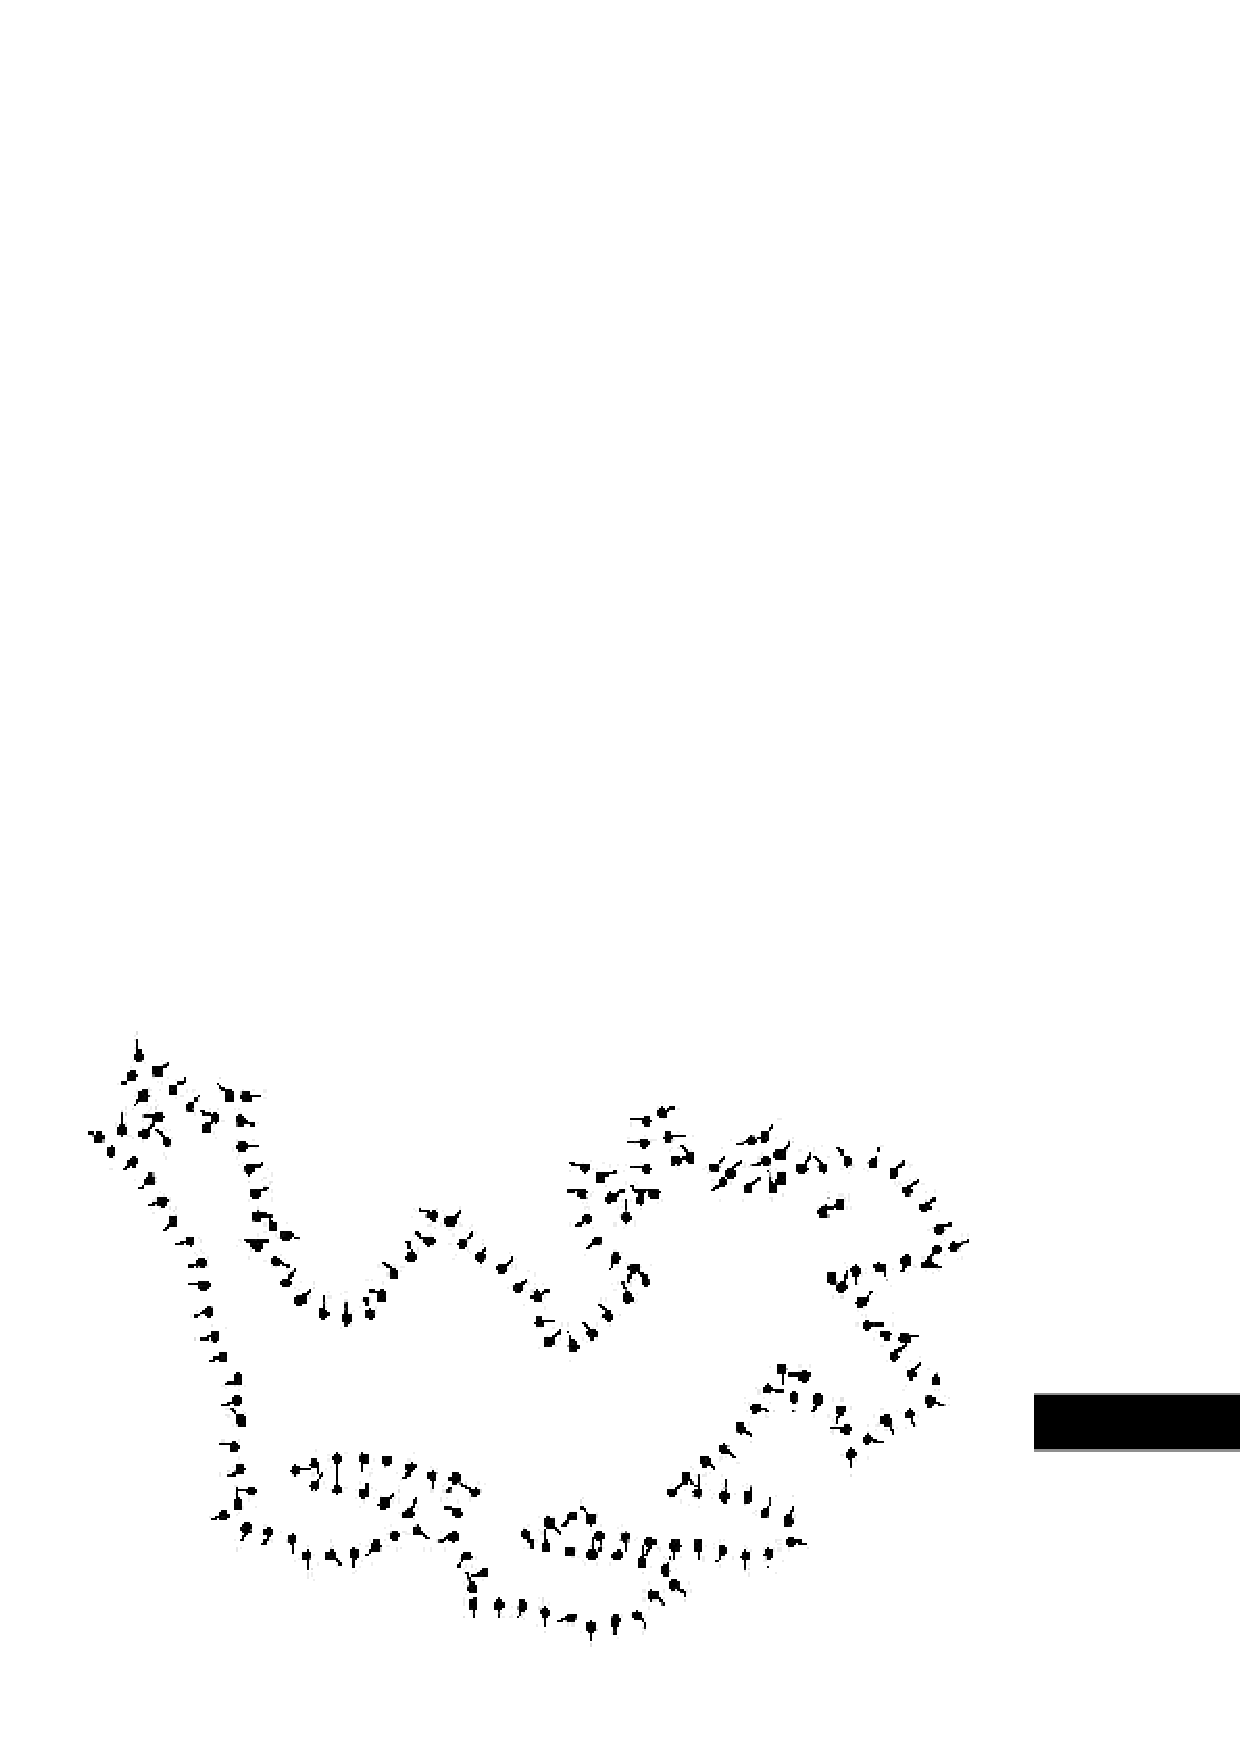
\includegraphics[width=0.7\textwidth]{Surface_reconstruction_3/clustering} % omit .eps suffix
    \end{ccTexOnly}
    \begin{ccHtmlOnly}
        <img width="70%" border=0 src="../Surface_reconstruction_3/clustering.jpg"><P>
    \end{ccHtmlOnly}
    % Title
    \begin{figure}[h]
        \caption{Point set simplification by clustering}
    \end{figure}
\end{center}

The \ccc{CGAL::merge_epsilon_nearest_points_3()} function exists in four flavors.
First, the function may modify the input point set or create a copy.
Second, the function may require the kernel to use for computations, or deduce it from input parameters.

\ccInclude{CGAL/merge_epsilon_nearest_points_3.h}

% The section below is automatically generated. Do not edit!
%START-AUTO(\ccDefinition)

\ccFunction{OutputIterator merge_epsilon_nearest_points_3(InputIterator first, InputIterator beyond, OutputIterator output, double epsilon, const Kernel& );}
{
Merge points which belong to the same cell of a grid of cell size = epsilon. This variant requires the kernel.
Precondition: epsilon $>$ 0.
}
\ccGlue
\begin{description}
\item[Template Parameters:]
\begin{description}
\item[InputIterator]\ccc{value_type} must be convertible to OutputIterator's \ccc{value_type}. \item[OutputIterator]\ccc{value_type} must be convertible to \ccc{Point_3}. \item[Kernel]Geometric traits class.\end{description}
\end{description}
\begin{description}
\item[Returns:]past-the-end output iterator. \end{description}
\begin{description}
\item[Parameters: ]
\begin{description}
\item[first]input points \item[output]output points \item[epsilon]tolerance value when comparing 3D points \end{description}
\end{description}
\ccGlue
\ccFunction{ForwardIterator merge_epsilon_nearest_points_3(ForwardIterator first, ForwardIterator beyond, double epsilon, const Kernel& );}
{
Merge points which belong to the same cell of a grid of cell size = epsilon. This function is mutating the input point set. This variant requires the kernel.
Warning: This method modifies the order of points, thus should not be called on sorted containers.
Precondition: epsilon $>$ 0.
}
\ccGlue
\begin{description}
\item[Template Parameters:]
\begin{description}
\item[ForwardIterator]\ccc{value_type} must be convertible to \ccc{Point_3}. \item[Kernel]Geometric traits class.\end{description}
\end{description}
\begin{description}
\item[Returns:]First iterator to remove (see erase-remove idiom). \end{description}
\begin{description}
\item[Parameters: ]
\begin{description}
\item[first]input/output points \item[epsilon]tolerance value when comparing 3D points \end{description}
\end{description}
\ccGlue
\ccFunction{OutputIterator merge_epsilon_nearest_points_3(InputIterator first, InputIterator beyond, OutputIterator output, double epsilon);}
{
Merge points which belong to the same cell of a grid of cell size = epsilon. This variant deduces the kernel from iterator types.
Precondition: epsilon $>$ 0.
}
\ccGlue
\begin{description}
\item[Template Parameters:]
\begin{description}
\item[InputIterator]\ccc{value_type} must be convertible to OutputIterator's \ccc{value_type}. \item[OutputIterator]\ccc{value_type} must be convertible to \ccc{Point_3}.\end{description}
\end{description}
\begin{description}
\item[Returns:]past-the-end output iterator. \end{description}
\begin{description}
\item[Parameters: ]
\begin{description}
\item[first]input points \item[output]output points \item[epsilon]tolerance value when comparing 3D points \end{description}
\end{description}
\ccGlue
\ccFunction{ForwardIterator merge_epsilon_nearest_points_3(ForwardIterator first, ForwardIterator beyond, double epsilon);}
{
Merge points which belong to the same cell of a grid of cell size = epsilon. This function is mutating the input point set. This variant deduces the kernel from iterator types.
Warning: This method modifies the order of points, thus should not be called on sorted containers.
Precondition: epsilon $>$ 0.
}
\ccGlue
\begin{description}
\item[Template Parameters:]
\begin{description}
\item[ForwardIterator]\ccc{value_type} must be convertible to \ccc{Point_3}.\end{description}
\end{description}
\begin{description}
\item[Returns:]First iterator to remove (see erase-remove idiom). \end{description}
\begin{description}
\item[Parameters: ]
\begin{description}
\item[first]input/output points \item[epsilon]tolerance value when comparing 3D points \end{description}
\end{description}
\ccGlue

%END-AUTO(\ccDefinition)

\ccParameters

The full template declarations are:

% The section below is automatically generated. Do not edit!
%START-AUTO(\ccParameters)

template$<$  \\
typename InputIterator,   \\
typename OutputIterator,   \\
typename Kernel$>$  \\
OutputIterator  \\
\ccc{merge_epsilon_nearest_points_3} (InputIterator first, InputIterator beyond, OutputIterator output, double epsilon, const Kernel\& );  \\
  \\
template$<$  \\
typename ForwardIterator,   \\
typename Kernel$>$  \\
ForwardIterator  \\
\ccc{merge_epsilon_nearest_points_3} (ForwardIterator first, ForwardIterator beyond, double epsilon, const Kernel\& );  \\
  \\
template$<$  \\
typename InputIterator,   \\
typename OutputIterator$>$  \\
OutputIterator  \\
\ccc{merge_epsilon_nearest_points_3} (InputIterator first, InputIterator beyond, OutputIterator output, double epsilon);  \\
  \\
template$<$  \\
typename ForwardIterator$>$  \\
ForwardIterator  \\
\ccc{merge_epsilon_nearest_points_3} (ForwardIterator first, ForwardIterator beyond, double epsilon);  \\

%END-AUTO(\ccParameters)

\ccSeeAlso

\ccRefIdfierPage{random_simplification_points_3}  \\

\ccExample

\begin{ccExampleCode}
typedef CGAL::Exact_predicates_inexact_constructions_kernel Kernel;
typedef Kernel::Point_3 Point;
std::deque<Point> points = ...;
double epsilon = 0.001;

// put result in output iterator...
std::deque<Point> output;
CGAL::merge_epsilon_nearest_points_3(points.begin(), points.end(),
                                     std::back_inserter(output),
                                     epsilon);

// ...or use mutating version of the same function
std::deque<Point>::iterator first_iterator_to_remove =
  CGAL::merge_epsilon_nearest_points_3(points.begin(), points.end(),
                                       epsilon);
std::erase(std::remove(first_iterator_to_remove, points.end()), // erase-remove idiom
           points.end());
\end{ccExampleCode}

\end{ccRefFunction}

% +------------------------------------------------------------------------+
%%RefPage: end of main body, begin of footer
\ccRefPageEnd
% EOF
% +------------------------------------------------------------------------+

